\documentclass[10pt]{article}
\usepackage[utf8]{inputenc}
\usepackage[T1]{fontenc}
\usepackage{PRIMEarxiv}
\usepackage{titlesec}
\usepackage{amsmath}
\usepackage{amsfonts}
\usepackage{amssymb}
\usepackage{mhchem}
\usepackage{stmaryrd}
\usepackage{graphicx}
\usepackage[export]{adjustbox}
\graphicspath{ {./images/} }
\usepackage{hyperref}
\hypersetup{colorlinks=true, linkcolor=blue, filecolor=magenta, urlcolor=cyan,}
\urlstyle{same}


%Header
\pagestyle{fancy}
\thispagestyle{empty}
\rhead{ \textit{ }} 

% Update your Headers here
%\fancyhead[LO]{Running Title for Header}
% \fancyhead[RE]{Firstauthor and Secondauthor} % Firstauthor et al. if more %than 2 - must use \documentclass[twoside]{article}



  
%% Title
\title{Quantum-Classical Hybrid Neural Networks for Image Classification using a PyTorch-Qiskit based pipeline
%%%% Cite as
%%%% Update your official citation here when published 


}
%\author{
%Rita Abani
%}
\author{
  Rita Abani \\
  Department of Electrical Engineering and Computer Science \\
  Indian Institute of Science Education and Research, Bhopal \\
  Bhopal, India\\
  %\texttt{\{Author1, Author2\}email@email} \\
  %% examples of more authors
   %\And
  %Author3 \\
  %Affiliation \\
  %Univ \\
  %City\\
  %\texttt{email@email} \\
  %% \AND
  %% Coauthor \\
  %% Affiliation \\
  %% Address \\
  %% \texttt{email} \\
  %% \And
  %% Coauthor \\
  %% Affiliation \\
  %% Address \\
  %% \texttt{email} \\
  %% \And
  %% Coauthor \\
  %% Affiliation \\
  %% Address \\
  %% \texttt{email} \\
}


\begin{document}
\maketitle


\begin{abstract}
Conventional Machine learning algorithms have given rise to interesting ideas and utilities that have made analysis of big data, image classification etc. efficient. However, with the recent turn of events in the domain of Quantum Computation and Quantum Technology, the possibility of using Quantum Machine Learning to boost and ameliorate various data analysis or optimization dependent tasks has been an active and inter-disciplinary area of research. Leveraging the principles of Quantum Mechanics namely Entanglement, Superposition, and the concept of parallelism, quantum computers are hypothesized to tackle the paucity created by the gradual saturation of Moore's Law. In this paper, the author wishes to study the application of partially quantized classical neural networks or Hybrid-Quantum Classical Neural Networks in the field of Image Classification and gauge how lucrative variational circuits can prove to be as classifiers.
\end{abstract}


% keywords can be removed
%-\keywords{First keyword \and Second keyword \and More}


\section{Introduction}
The importance of supervised machine learning has only augmented in the past few years given the sudden boom in the big data industry. With the unprecedented requirement of tools to handle copious amounts of data comes the need to explore alternatives to existing classical hardware and software. Quantum Computation has hence been viewed as a factor that could change the current pace of data handling. Quantum Computing harnesses the principles of Quantum Mechanics namely superposition and entanglement to perform calculations. In this work, we explore the use of a Hybrid quantum-classical Neural Network model built using the PyTorch-Qiskit framework. Feed Forward Neural Networks is the type of Neural Network deployed in this work that can be described using the Directed Acyclic Graph (DAG). We make use of the parameter shift rule [1] to calculate the gradient of quantum circuit parameters ( which is needed to employ gradient descent for optimisation). Since this is a Hybrid network, we employ a sandwich structure wherein a hidden layer for the conventional neural network is replaced by a parametrized quantum circuit.

This paper also explores the ease of integrating Qiskit with PyTorch which is an optimized tensor library primarily used for Deep Learning applications using GPUs and CPUs.

The dataset used to perform the study is the CIFAR-10 dataset which can be easily accessed from the Torchvision library of the PyTorch framework. The dataset consists of $6000032 \times 32$ colour images in 10 classes, with 6000 images per class. There are 50000 training images and 10000 test images. In this study, a quantum classical hybrid neural network was used to build a binary classifier that could distinguish between images of Aeroplanes and Automobiles. The study could be extended further to make a multi-classifier (but that is out of the scope of this paper).


%\section{Related work}


\subsection{Network Architecture}
In a neural network, a neuron is analogous to a mathematical nonlinear function which maps one or more than one inputs to a single real number. Graphically neurons are represented as nodes in a graph and directed edges are drawn between nodes to indicate how the output of one neuron can be used or fed as an input to the other neurons. Each edge in the graph is associated with a scalar valued 'weight'. In our model, a Feed Forward Neural Network was used. A Feed Forward Neural Network is a type of Artificial Neural Network where connections between nodes do not form a cycle or in other words, we will have a unidirectional flow of data in our model.

In this model of the quantum classical neural network, there is an input layer, a hidden layer and an output layer. The first and the last layers are classical in nature while the hidden layer implements the quantum component of our model in the form of a Parametrized Quantum Circuit. The PQC is a quantum circuit where rotation angles for each gate are specified using components from a classical input vector. Optimization techniques are necessary to update the model parameters. A question that might arise is how the gradients of a PQC could be calculated. In our model, we use the 'Parameter Shift Rule' [1] to measure the gradients of the PQC with respect to its parameters.

Since the network model leverages the Qiskit-PyTorch pipeline, it becomes efficient to put all the Qiskit Quantum functions into a class by first specifying how many trainable quantum parameters and shots are required. In this model we use a 1 -qubit circuit with $\theta$ as our trainable parameter.

Similar to the approach used in the Qiskit textbook, [2] the circuit is then hard coded for simplicity and then an RY rotation is performed by an angle of $\theta$ so as to train the output of the circuit. The back end framework of the Quantum Class is depicted in Figure 1

\begin{figure}
    \centering
    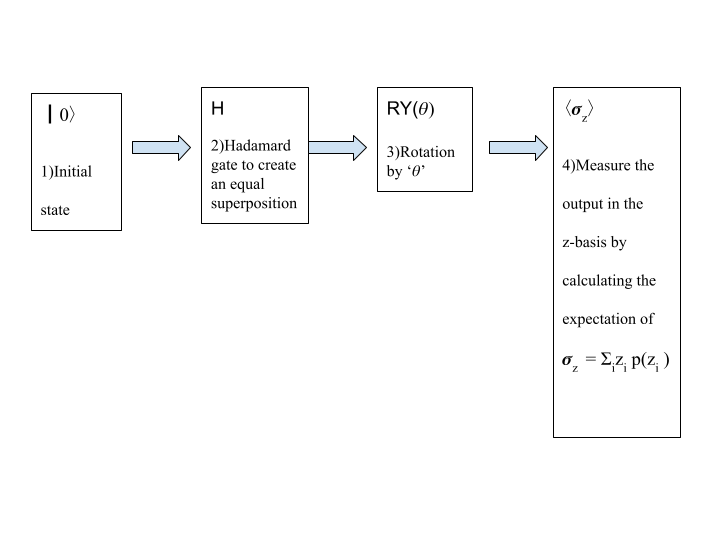
\includegraphics[width=15cm, height=11cm]{elias flowchart.png}
    \caption{ Back-end framework of the Quantum Circuit describing the quantum layer and the process of measurement.}
    \label{fig:my_label}
\end{figure}


Post defining the Quantum circuit, the functions required to tune the quantum-classical layer were implored. The functions required for backpropagation are coded using PyTorch while the forward and backward passes are defined using elements from Qiskit. Using the Parameter Shift rule, the backward pass directly computes the analytical gradients.

The process of loading data and preprocessing first involved loading the CIFAR-10 dataset  $[\underline{3}]$ from the Torchvision datasets and then filtering for the pictures of automobiles and aeroplanes. These filtered pictures serve as an input to the hybrid neural network to classify. The number of datapoints per class, i.e aeroplanes and automobiles were specified.

It is worthwile to note that solely evaluating a model on the training dataset would result in some amount of bias, therefore the model was evaluated on a held-out sample (unseen data) as well to give a fairly unbiased estimate of accuracy. This approach of the train-test split termed 'hold-out validation' has been used in the code. Using the random\_split feature from torch.utils.data, the cifar\_trainset was split into a validation set and a train set.

\subsection{Construction of the Hybrid Network:}

A PyTorch-Qiskit pipeline was deployed to create the architecture of the neural network. For mathematical consistency, the network had to be consistent in terms of its dimensionality when adding the Parametrized Quantum Circuit. Since the model in this paper had chosen 1 parameter, it was ensured that the network condensed neurons down to size 1 and then the usual Convolutional Neural Network with two fully connected layers at the end (the model was also experimented with by altering the layers, adding and changing dropout, max\_pool2d etc. so as to ascertain the effect of these factors towards the test accuracy). The input to the Quantum circuit is fed in the form of the parameter ' $\theta$ ' which is technically the value of the last neuron of the fully connected layer. The circuit measurement or the expectation about the z-basis serves as the final prediction whether the image is an 'aeroplane' or an 'automobile'. 

\subsection{Network training and testing:}

Training the network involved experimenting with the best permutations of optimizer, learning rate and loss function as hyperparameters in order to train over multiple epochs and validate the same. Hyperparameter tuning was carried out. The network was first trained on the training sample, it was then validated so as to determine whether the model suffered through under-fitting or over-fitting. Before determining the test accuracy, the layers were altered to determine the best possible layer architecture alongside the best combination of hyperparameters. The following are the different model structures that were analysed subsequently:
\subsection{Model 1 : The standard reference model}
PyTorch tools were used to create the hybrid. A typical CNN with two fully connected layers at the end was made. The value of the last neuron of the fully connected layer is fed as the ' $\theta$ ' to the parametrized Quantum Circuit

Optimizer: Adam, Learning rate: 0.001, Loss function: Negative Log Likelihood NLLLoss O\\

\includegraphics[max width=\textwidth]{2022_06_02_204e286de780e5525edcg-07}

Number of Epochs : 20    \hspace{19em}  Number of Epochs: 30

Test Accuracy : $80.5 \%$   \hspace{19em}  Test Accuracy: $80.0 \%$\\

\includegraphics[max width=\textwidth]{2022_06_02_204e286de780e5525edcg-08}

Number of Epochs : 40  \hspace{19em}  Number of Epochs: 50

Test Accuracy : 81.0\%   \hspace{19em} Test Accuracy : $47.5 \%$ \\

As can be seen from the above graphs, the loss curves don't provide a conducive picture on reducing overfitting. Furthermore, they do not converge on increasing the number of epochs. While the test accuracy in $20,30,40$ epochs showed promise, when raised to 50 , the curves did not seem to converge or follow noteworthy training. This implies the need to check using changes in learning rate or a different network structure.

It was experimentally determined that the optimum parameters for this include Adam as the optimiser and a learning rate of around $0.0001$ to $0.0005$ with 15 epochs.
\setlength{\parskip}{1pt}
\subsection{Model 2:}
Layers added: F.max\_pool2d( $x$, 2),self.dropout $(x)$

Optimizer: Adam , Learning rate: 0.001, Loss function: Negative Log Likelihood NLLLoss(

Other loss functions like CrossEntropyLoss() were experimented with, but did not prove to be as efficient as NLLLoss() In the forward function, a max\_pool2D() layer was applied.

max\_pool2d( $\mathrm{x}, 2)$ as we know applies a 2D max pooling over an input signal composed of several input planes. This approach was tried because the output after max-pooling layer would be a feature map containing the most prominent features of the previous feature map.

Additionally, another dropout layer was added self.dropout( $x$ ) to check if overfitting could be regulated.During training, the dropout function randomly zeroes some of the elements of the input tensor with probability 'p' using samples from a Bernoulli distribution.\\

\includegraphics[max width=\textwidth]{2022_06_02_204e286de780e5525edcg-09}

Number of Epochs: 30 \hspace{19em} Number of Epochs : 40 

Test Accuracy : 73.0\%  \hspace{19em}  Test Accuracy : 73.5\% \\




Optimal Test Accuracy : 73.0\% \\
As can be seen from the above graphs, neither the accuracy nor the convergence of the curves seems encouraging. The chaotic curves imply that having 2 dropout layers in the forward function not only bring down the training accuracy but also are not substantial enough to curb overfitting or reduce validation loss.

\subsection{Model 3:}
Layers added: F.max pool2d $(x, 2)$, self.dropout $(x)$, torch.flatten $(x, 1)$ Optimizer: Adam, Learning rate: 0.001, Loss function: Negative Log Likelihood NLLLoss()

Building up on Model 2 , torch.flatten $(x, 1)$ was added to it. Torch.flatten $(x, 1)$ flattens the input by reshaping it into a one-dimensional tensor. Only dimensions starting with $\mathrm{x}$ and ending with 1 are flattened and hence the order of elements in input is unchanged.\\

\includegraphics[max width=\textwidth]{2022_06_02_204e286de780e5525edcg-10}

Number of Epochs : 5   \hspace{19em}  Number of Epochs: 20

Test Accuracy : 51.0\%  \hspace{19em}  Test Accuracy : $72.0 \%$\\

\includegraphics[max width=\textwidth]{2022_06_02_204e286de780e5525edcg-11}

Number of Epochs : 30 \hspace{19em} Number of Epochs: 40

Test Accuracy : 77.5\% \hspace{19em} Test Accuracy : 79.0\% \\

The use of torch.flatten $(x, 1)$, coupled with the dropout seems to have improved the convergence of the loss curve and minimized the difference between validation loss and training loss.

Though this has brought down the overall test accuracy, the overall validation loss has improved. This accounts for a lower generalization error.

\subsection{Model 4:}
\vspace{-\lineskip}
\newline



In this network, the dropout layer was removed (considering that the number of samples is small and that this is a binary classification problem, and hence there is a chance that the dropout layer could have brought down the training accuracy).

Though the dropout layer is hypothesized to reduce the generalization error, it seemed logical to test the model without it.\\

\includegraphics[max width=\textwidth]{2022_06_02_204e286de780e5525edcg-12}

Number of Epochs $: 5$  \hspace{19em}  Number of Epochs: 20

Test Accuracy : 76.5\%  \hspace{19em}  Test Accuracy : $80.5 \%$\\



\includegraphics[max width=\textwidth]{2022_06_02_204e286de780e5525edcg-12(1)}

Number of Epochs : 30  \hspace{19em}  Number of Epochs: 40

Test Accuracy : $83.5 \%$  \hspace{19em} Test Accuracy : 76.5\% \\



This model seemed to show encouraging convergence in the loss curves along with an optimum accuracy of $83.5 \%$ with 30 epochs. The classical counterpart of the same model with 30 epochs showed an accuracy of $80.1 \%$. Hence the Quantum model showed an advantage over the Classical model in a few cases.

The same model was hence tried using a learning rate of $0.0005$ which showed very encouraging loss curves with a fairly promising accuracy on the test data.

\includegraphics[width=9cm]{2022_06_02_204e286de780e5525edcg-13}

Number of Epochs : 30

Test Accuracy : $80.5 \%$

Learning rate $\mathbf{0 . 0 0 0 5}$
\section{Effect of using a Hardware accelerator to enhance the test accuracy of the model:}

The code for the model was run on both a GPU Hardware accelerator ( Google Colaboratory's backend cloud version ) and the cloud CPU. The test accuracies were closely monitored.

Considering the Model 4 (which showed encouraging capacity and accuracy) with 30 epochs, Adam Optimizer and a learning rate of $0.0005$ we get the following:\\

\includegraphics[max width=\textwidth]{2022_06_02_204e286de780e5525edcg-14}
%Number of Epochs $: 5$  \hspace{10em}  Number of Epochs: 20
  



Nvidia Tesla K80 GPU \hspace{8em}      Intel(R) Xeon(R) CPU @ 2.30GHz \\

Test Accuracy : 80.5\%  \hspace{10em}  Test Accuracy : $78.0 \%$\\

Execution time : 207.285 s \hspace{8em}   Execution time: 215.295s  


%\subsection{Nvidia Tesla K80 GPU}
%Intel( $\mathrm{R}) \mathrm{Xeon}(\mathrm{R}) \mathrm{CPU}$ @. $20 \mathrm{GHz}$

%Test Accuracy: $80.5 \%$

%Test Accuracy :78.0\%

%Execution time : $207.285$ seconds

%Execution time: $215.295 \mathrm{~s}$

Hence, it was tdeduced that for a good model that fairly doesn't suffer from bias, using a hardware accelerator like the GPU does not give a significant advantage with respect to test accuracy (in this case there is a difference of $2.5 \%$ ). It does however give an edge over the execution time by a few seconds (in this case there was a difference of $7.9445$ seconds).

However in the case of a few models, where there seemed to be overfitting or bias in other parameters, GPU as a hardware accelerator showed substantial improvement in accuracy by a margin of about $6.5 \%$ like in the case below of Model 1 with a learning rate of $0.001$, Adam as the optimizer, 30 epochs and Negative Log Likelihood Loss as the Loss function.

\begin{figure}[!h]

\includegraphics[max width=\textwidth]{images/s1.PNG}
\includegraphics[max width=\textwidth]{images/s2.PNG}
Intel $(\mathrm{R}) \mathrm{Xeon}(\mathrm{R}) \mathrm{CPU} @ 2.30 \mathrm{GHz}$ \hspace{11em} Nvidia Tesla K80 GPU



\end{figure}

Link to the GitHub repository for this project : \href{https://github.com/DRA-chaos/Quantum-Classical-Hyrid-Neural-Network-for-binary-image-classification-using-PyTorch-Qiskit-pipeline}{https://github.com/DRA-chaos/Quantum-Classical-Hyrid-Neural-Network-for-binary-image-classification-using-PyTorch-Qiskit-pipeline}



\section{CONCLUSION}
We have demonstrated the possibility of creating an image classifier using hybrid neural networks. The integration of PyTorch and Qiskit helps amalgamate techniques from both classical ML and Quantum Computing. However, this was more of a simplistic model, the code used has scope to be extended to other branches of study like for example Astronomy (like classification of astronomical transients), problems in high energy physics, gene sequencing etc. Considering the paucity caused by the gradual saturation of Moore's Law, it has become quintessential to explore alternatives like Quantum Neural Networks or Hybrid Neural Networks, though significant work is still left in reaching a mathematically conducive model of a Quantum Perceptron [7]. Finding the correct quantum generalisation of the perceptron, the right neural network model, optimisation algorithm and loss function are crucial in ensuring the model performs well.

\section{ACKNOWLEDGEMENTS}

The author would like to thank Dr Elias F Combarro , Associate Professor , Quantum and High Performance Computing Group, Universidad de Oviedo , Spain for his guidance.
\section{REFERENCES:}
[1]Crooks, Gavin. (2019). Gradients of parameterized quantum gates using the parameter-shift rule and gate decomposition. \href{https://arxiv.org/pdf/1905.13311.pdf}{https://arxiv.org/pdf/1905.13311.pdf}

[2]A. Asfaw, L. Bello, Y. Ben-Haim, S. Bravyi, L. Capelluto, A. C. Vazquez, J. Ceroni, J.

Gambetta, S. Garion, L. Gil, et al., Learn quantum computation using qiskit (2020), URL:\href{https://qiskit.org/textbook/ch-machine-learning/machine-learning-qiskit-pytorch.html}{https://qiskit.org/textbook/ch-machine-learning/machine-learning-qiskit-pytorch.html}

[3]Krizhevsky, Alex. (2012). Learning Multiple Layers of Features from Tiny Images. University of Toronto. \href{https://www.cs.toronto.edu}{https://www.cs.toronto.edu} $/ \sim$ kriz/cifar.html

[4]Oh, Seunghyeok \& Choi, Jaeho \& Kim, Joongheon. (2020). A Tutorial on Quantum Convolutional Neural Networks (QCNN).\href{https://arxiv.org/pdf/2009.09423.pdf}{https://arxiv.org/pdf/2009.09423.pdf}

[5]Farhi, Edward \& Neven, Hartmut. (2018). Classification with Quantum Neural Networks on Near Term Processors. \href{https://arxiv.org/pdf/1802.06002.pdf}{https://arxiv.org/pdf/1802.06002.pdf}

[6]Kulkarni, Viraj \& Kulkarni, Milind \& Pant, Aniruddha. (2020). Quantum Computing Methods for Supervised Learning. \href{https://arxiv.org/pdf/2006.12025.pdf}{https://arxiv.org/pdf/2006.12025.pdf}

[7]Beer, K., Bondarenko, D., Farrelly, T. et al. Training deep quantum neural networks. Nat Commun 11, 808 (2020). \href{https://doi.org/10.1038/s41467-020-14454-2}{https://doi.org/10.1038/s41467-020-14454-2}

[8]Cong, Iris \& Choi, Soonwon \& Lukin, Mikhail. (2019). Quantum convolutional neural networks. Nature Physics. 15. 1-6. 10.1038/s41567-019-0648-8.

\href{https://arxiv.org/pdf/1810.03787.pdf}{https://arxiv.org/pdf/1810.03787.pdf}


\end{document}